\documentclass[a4paper,12pt,fleqn]{article}
\usepackage{fixltx2e}
\usepackage[utf8]{inputenc}
\usepackage{graphicx}
\usepackage{sidecap}
\usepackage{fancyhdr}
\usepackage{amssymb,mathtools}
\usepackage[swedish]{babel}
\usepackage[margin=1.5in]{geometry}
\usepackage{abstract}
\usepackage[parfill]{parskip}
\usepackage{tocloft}
\usepackage{adjustbox}
\usepackage{textcomp}
\usepackage[T1]{fontenc}
\usepackage{listings}
\usepackage{xcolor,colortbl}
\usepackage{hyperref}

%----------------------------------------------------------------
%C-kod formatering

\definecolor{listinggray}{gray}{0.9}
\definecolor{lbcolor}{rgb}{0.9,0.9,0.9}
\lstset{
backgroundcolor=\color{lbcolor},
    tabsize=4,    
%   rulecolor=,
    language=[GNU]C++,
        basicstyle=\scriptsize,
        upquote=true,
        aboveskip={1.5\baselineskip},
        columns=fixed,
        showstringspaces=false,
        extendedchars=false,
        breaklines=true,
        prebreak = \raisebox{0ex}[0ex][0ex]{\ensuremath{\hookleftarrow}},
        frame=single,
        numbers=left,
        showtabs=false,
        showspaces=false,
        showstringspaces=false,
        identifierstyle=\ttfamily,
        keywordstyle=\color[rgb]{0,0,1},
        commentstyle=\color[rgb]{0.026,0.112,0.095},
        stringstyle=\color[rgb]{0.627,0.126,0.941},
        numberstyle=\color[rgb]{0.205, 0.142, 0.73},
%        \lstdefinestyle{C++}{language=C++,style=numbers}’.
}
\lstset{
    backgroundcolor=\color{lbcolor},
    tabsize=4,
  language=C++,
  captionpos=b,
  tabsize=3,
  frame=lines,
  numbers=left,
  numberstyle=\tiny,
  numbersep=5pt,
  breaklines=true,
  showstringspaces=false,
  basicstyle=\footnotesize,
%  identifierstyle=\color{magenta},
  keywordstyle=\color[rgb]{0,0,1},
  commentstyle=\color{Darkgreen},
  stringstyle=\color{red}
  }
  %-----------------------------------------------------------------
  %marginaler

  \renewcommand{\abstractnamefont}{\normalfont\normalsize\bfseries}
  \renewcommand{\abstracttextfont}{\normalfont\small}
  \renewcommand{\headrulewidth}{0pt}
  \renewcommand{\cftsecleader}{\cftdotfill{\cftdotsep}} 
  \setlength{\absleftindent}{0pt}
  \setlength{\absrightindent}{0pt}
  \setlength{\headheight}{15pt}

  \addtolength{\oddsidemargin}{-.5in}
  	\addtolength{\evensidemargin}{-.5in}
  	\addtolength{\textwidth}{1in}


  %-----------------------------------------------------------------
  %header and footer

  \pagestyle{fancy}
  \lhead{
  	\begin{picture}(0,0)
  		\put(5,0){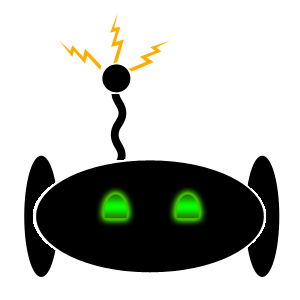
\includegraphics{logotyp.png}}
  	\end{picture}}
	
  \fancyhead[C]{\small{Mapmaster2001}}
  \fancyhead[R]{\small \today}
  \fancyfoot[L]{\small{TSEA56 \\ LIPS Kappa}}
  \fancyfoot[C]{\small{\thepage}}
  \fancyfoot[R]{\small{Projektgrupp 8 \\ mapmaster2001@cyd.liu.se}}

  %-----------------------------------------------------------------

%-------------------------------------------------------------------
%Första sidan

\begin{document}
	\pagestyle{fancy}
	 \pagenumbering{gobble}
	\vspace*{\fill}
		\begingroup
			\begin{center}
				\huge{\textbf{Simultan positionering och kartläggning}}
				\\
				\vspace{10pt}
				\normalsize
				Tobias Grundström och Hans-Filip Elo
				\\
				Kandidatprojekt Y - Grupp 8 - VT2014
				\\
				Version 0.2
				\end{center}
		\endgroup
	\vspace*{\fill}

	\begin{center} %Börjar centrering 
		Status
		\\
		\vspace{3pt} %Whitespace 3 pts
	    \begin{tabular}{| p{3cm} | p{3cm} | p{3cm} |} %tabell, 4 horizontella |, 3 cm emellan dem.
	    \hline %översta horizontella linjen.
	    Granskad & hanel742 & \today \\ \hline % & -tecken för att "gå till nästa ruta" 
		Godkänd & - & - \\ \hline % avslutas med \\ och \hline.

	    \end{tabular}
	\end{center}
	\vspace{2cm}
	\newpage
%-----------------------------------------------------------------
%Projektidentitet


	\vspace*{\fill}
		\begingroup
			\begin{center}
				\pagenumbering{roman}
				\LARGE{\textbf{PROJEKTIDENTITET}}
				\\
				\footnotesize
				Grupp 8, 2014/VT, MapMaster2001
				\\
				Linköpings tekniska högskola, Institutionen för Systemteknik (ISY)
				\\
				\vspace{1cm}
	  \begin{tabular}{| p{3cm} | p{4.3cm} | p{2.4cm} | p{3.8cm} |}
	    \hline
		\textbf{Namn} & \textbf{Ansvar} & \textbf{Telefon} & \textbf{E-post} \\ \hline
	    Jens Edhammer & Dokumentanvsvarig (DOK) & 076-030 67 80 & jened502@student.liu.se \\ \hline
		Erik Ekelund & Designansvarig (DES) & 073-682 43 06 & eriek984@student.liu.se \\ \hline
		David Habrman &  & 976-017 71 15 & davha227@student.liu.se \\ \hline 
		Tobias Grundström & Testansvarig (TES) & 073-830 44 45 & tobgr602@student.liu.se \\ \hline 
		Hans-Filip Elo &   & 073-385 22 32 & hanel742@student.liu.se \\ \hline 
		Niklas Ericson & Projektledare (PL) & 073-052 27 05 & niker917@student.liu.se \\ \hline
	    \end{tabular}

		\vspace{1cm}
		\textbf{E-postlista för hela gruppen:} mapmaster2001@cyd.liu.se
		\\[0.5cm]

		\textbf{Kund}: Mattias Krysander, Linköpings universitet, 581 83  LINKÖPING, \\
		013-28 21 98, matkr@isy.liu.se \\
		\textbf{Kontaktperson hos kund}: Mattias Krysander, 013-28 21 98,matkr@isy.liu.se 
		\\
		\textbf{Kursansvarig}: Tomas Svensson, 3B:528,013 28 21 59,tomass@isy.liu.se
		\\[0.5cm]
		\textbf{Handledare}: Peter Johansson, 013-28 1345 peter.a.johansson@liu.se

				\end{center}
		\endgroup
	\vspace*{\fill}
\newpage

%-----------------------------------------------------------------
%Innehållsföreteckning

\addto\captionsswedish{\renewcommand{\contentsname}{Innehållsförteckning}}

\tableofcontents
\thispagestyle{fancy}
\newpage

\pagenumbering{arabic}
%-----------------------------------------------------------------
%Översikt

%------------------------------------------------
%--------------------Inledning-------------------
%------------------------------------------------
\section{Inledning}

Simultan positionering och kartläggning (SLAM) är ett problem som grundar sig i följande frågeställning: Utan att veta var vi är - hur kartlägger vi då vår omgivning? Åt andra hållet får man ställa sig frågan - hur vet vi var vi befinner oss utan en karta?

Det är inte helt enkelt att lösa dessa frågor, men det finns approximativa lösningar på SLAM-problemet . Gemensamt för alla lösningar är att de bygger på möjligheten att läsa av sin omgivning i kombination med
sannolikhetsteori. Då sensordata aldrig kan antas vara exakt använder man sannolikhetsteori för att göra rimlighetsbedömningar i de stickprov av mätningar sensorerna ger.

SLAM-problemet är alltså oftast inte entydigt lösbart rent matematiskt, utan
bygger på sannolikhetsteori i kombination med att moderna processorer
och minnen kan hantera en stor mängd data. Moderna processorer möjliggör
alltså ett stort stickprov vilket kan leda till en mindre osäkerhet.

\subsection{Syfte}
Syftet med denna rapport är att ge läsaren en introduktion till de algoritmer och tekniker som används för kartläggning och positionsbestämning i ett mikroprocessorsystem och att lösa ett enklare SLAM-problem. 

\subsection{Historia}

Principerna för SLAM formulerades för första gången 1986\footnote{Smith, R.C.; Cheeseman, P. (1986).
''On the Representation and Estimation of Spatial Uncertainty''. The
International Journal of Robotics Research, 5(4), sida 56–68. Hämtad 28 mars 2014}. Redan vid formuleringen av problemet beskrevs SLAM som en inexakt vetenskap. SLAM handlar om att skaffa sig en approximativ uppfattning av sin omgivning och position som är tillräckligt bra för att fatta ett beslut kring färdväg och/eller kartläggning. 

Utvecklingen på området har sedan dess accelererat kraftigt tack vare
mikrokontrollers förmåga att hantera mer data. Då sannolikhetsberäkningarna SLAM innefattar gynnas kraftigt av att arbeta
med stora stickprov, hanterar 

På senare år har man, precis som inom många andra vetenskapliga områden, sett utvecklingen ta ytterligare ett kliv tack vare internet och öppna källkodsprojekt som Github och OpenSLAM. Att göra en sökning på ''SLAM'' på Github resulterar i en mängd aktiva projekt på området. Eftersom källkoden där också finns tillgänglig är detta ett utmärkt exempel för de som vill läsa på om SLAM-algoritmer. 

%------------------------------------------------
%-------------Problemformulering-----------------
%------------------------------------------------

\section{Problemformulering}

En robot med tillgång till ett antal avståndssensorer och ett gyro placeras i ett okänt slutet område. Den ska, med en vägg som startpunkt, helt autonomt kartlägga området genom att markera ut var väggar finns och var det finns områden som inte går att nå. Om inte hela det slutna området är kartlagt ska den upptäcka vilka segment som är oupptäckta, färdas dit och lägga till det i kartan. När området är kartlagt ska roboten ta sig tillbaka till startpunkten för att kunna återhämtas och på så sätt avsluta arbetet. 


%------------------------------------------------
%--------------------Fördjupning-----------------
%------------------------------------------------
\newpage
\section{Fördjupning}
I denna fördjupande del går vi igenom förkunskaper som krävs för att beskriva en implementering som kan utföra SLAM i en miljö lik den i problemställningen. 

%----------------------Odometri------------------
\subsection{Odometri}

För att kunna utföra SLAM krävs det att man gör odometri, det vill säga att man kontinuerligt uppskattar vägen som färdats. Odometri kan göras på olika sätt - exempelvis genom att optiskt mäta avstånd till objekt i sin omgivning, vinkelhastigheter på hjul med känd storlek eller steg med given längd. 

Många robotar nyttjar förmågan att optiskt mäta objekt i sin omgivning, men det förekommer även implementeringar med radar, sonar eller GPS. Det finns då möjlighet att kompensera för tidigare mätfel vid framtida mätningar, något som inte bara går att utföra med data från optiska sensorer, men som kan göra större inverkan på dessa. Om man enbart förlitar sig på interna mätningar finns risken att tidiga mätfel görs, vilket fortplantar sig och leder till än större felskattningar senare under kartläggningen. 
Uppskattandet av färdvägen är aldrig en exakt lära. Det finns alltid en viss osäkerhet i sensorer. Det är av denna anledning som SLAM är en sannolikhetslära mer än en exakt vetenskap. 

Med optisk avläsning av omvärlden finns alltid möjligheten att korrigera tidigare felaktiga mätvärden genom att samla in mer mätdata för att på ett korrektare sätt kunna beskriva sin omgivning. Av den anledningen är all typ av SLAM beroende av att på något sätt granska sin omgivning. 

\newpage

\subsection{Tillståndsrepresentation av reglersystem}

Inom reglerteknik kan linjära system beskrivas på så kallad tillståndsformel så som Glad och Ljung\footnote{Glad, Torkel och Ljung, Lennart (2006), \textit{Reglerteknik - Grundläggande teori}.} beskriver. I fallet med SLAM för en robot använder man robotens position som tillstånd , tecknat $\vec{x}$. En observatör används för att skatta positionen i förhållande till kringliggande objekt med hjälp av till exempel sensorvärden. Tillstånden mäts med tidsdiskreta värden då datorer endast hanterar diskreta mätningar och ej kontinuerliga. En diskret tillståndsbeskrivning av ett linjärt reglersystem beskrivs av: 

\begin{gather}
\vec{x}[n+1] = A\vec{x}[n] + B\vec{u}[n] \\
\vec{y}[n] = C\vec{x[n]} + D\vec{u[n]}
\end{gather}
\\
där $A$, $B$, $C$ och $D$ är matriser, $u$ är insignal och $\vec{y}$ exempelvis är kringliggande objekts position i förhållande till roboten, alternativt robotens position vid mätning med GPS/GLONASS. 

I ett realiserbart system nyttjas sensorer med en viss osäkerhet. Man kan därmed enbart skatta systemets tillstånd och inte exakt beräkna dem. 

\subsubsection{Skattning av tillstånd}

Tillståndsvariablerna kan skattas med flera metoder utifrån tillgänglig mätdata. Om man utgår från att närliggande mätningar görs kring samma position för roboten kan mätningarna antas vara normalfördelade kring en viss längd. 

\begin{figure}[htp] %Placera här om det finns plats, annars så snart som möjligt, på toppen av en sida.
  \begin{center}
  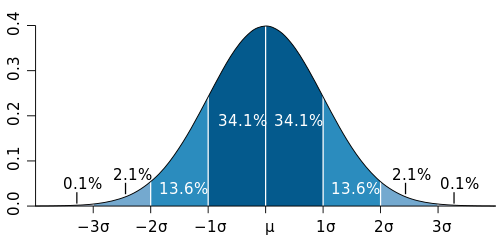
\includegraphics[keepaspectratio=true,scale=0.5]{normalfordelning.png}  %skala och filnamn. 
  \end{center}
  \caption{Normalfördelning} %figurtext.
  \label{fig:fire} %glöm inte att uppdatera era labels
\end{figure}

Variablernas tillstånd kan sedan skattas med mätningarnas väntevärde, $\mu$. Då mätningarna är normalfördelade ges väntevärdet av mätningarnas medelvärde, $\bar{x}$, vilket lätt ses i figur ovan\footnote{Wikipedia, \url{http://sv.wikipedia.org/wiki/Normalf\%C3\%B6rdelning}, hämtad 2014-05-02.}. 

Skattningen, alltså väntevärdet, är alltså observatören för tillståndsvariablerna i systemet. 

\newpage
%-------------------------------Typer av SLAM------------------------------------------------------
\subsection{Typer av SLAM}
Det finns olika typer av SLAM för olika typer av tillämpningar och med olika egenskaper. Vissa är bra på större områden medan andra är mer precisa och bra på mindre områden. 

\subsubsection{Kalmanfilter (KF-SLAM)}
Ett Kalmanfilter är en typ av algoritm som med hjälp av mätdata från sensorer, som kan innehålla brus och störningar, uppskattar okända variabler. Ett Kalmanfilter arbetar på linjära och oberoende tillståndsvariabler och är ett essentiellt verktyg för vägval samt positionsuppskattningen i ett SLAM-system. 

\subsubsection{EKF-SLAM} 
EKF-SLAM är en förkortning för Extended Kalman Filter for SLAM. Det utökade (extended) Kalmanfiltret skiljer sig från det ursprungliga på så vis att det används då tillståndsvariablerna ej kan antas vara linjära. Ett EKF linjäriserar variablerna kring ett medelvärde, och väger också in deras kovarians. Med kovarians menas här hur de olika variablernas varianser beror av varandra. Efter linjäriseringen appliceras sedan ett Kalmanfilter på variablerna.

\subsubsection{fastSLAM}
fastSLAM är en relativt modern teknik som använder ett så kallat partikelfilter för att filtrera givet mätdata, där varje värde i mätdatat ses som en partikel. De mest sannolika värdena sparas och de minst sannolika värdena förkastas. Man kallar det här för en omsapling av datat då man utgår från en sampelmängd av mätvärden och sedan minskar denna. 

För att effektivisera filtreringen av mätvärden delas olika distinkt upptäckta objekt i robotens miljö in i olika zoner. Dessa zoner filtreras sedan individuellt för att få fram den mest sannolika positionen för objektet i zonen. 

Mätvärdena körs sedan flera gånger genom filtret tills dess att man med tillräckligt stor sannolikhet kan bestämma kartans utseende. Metoden har visat sig väldigt effektiv i praktiken. Nackdelen med metoden är att man genom omsampling av mätvärdena förlorar mätinformation som skulle kunna vara korrekt. Beroende på hur filtret prioriterar är det möjligt att man får en skev bild av omgivningen. 

\subsection{Andra typer av sensorer}

I denna rapport berör vi mest området där SLAM baseras på optiska avståndssensorer, men det finns även andra typer av sensorer som går att använda. Nedan kommer några exempel på sådana implementeringar.

\subsubsection{VSLAM}

VSLAM står för visuell SLAM, vilket betyder att lokaliseringen sker med hjälp av kameror. Kamerorna används för att finna landmärken i området som kartläggs och sedan använda dessa som referenser när roboten fortsätter att utforska för att t ex se hur långt och i vilken riktning förflyttning sker relativt landmärket. Visuell SLAM är en förutsättning för att utnyttja den tidigare nämnda fastSLAM-tekniken. 

För att bedöma avstånd till ett objekt mäts vinklar mellan farkost och objektet vid olika tidpunkter. Utifrån farkostens hastighet kan mjukvaran sedan bestämma avståndet till objektet i fråga. 

VSLAM är i de allra flesta fall komplicerat att implementera då man behöver avancerade bildsökningsalgoritmer för att finna lämpliga landmärken. 

\subsubsection{TSLAM}
Tactile SLAM är en metod som provats för robotar vid kartläggning av ett mörklagt område. Metoden använder sig av känselsensorer för att hitta avgränsningar i området och med hjälp av detta rita upp kartan. Denna metod ger dock inte så bra resultat med de tekniker som existerar i dag.

\subsubsection{WiFi-SLAM}
Denna metod använder sig av styrkan på WiFi-signaler i närheten för att avgöra positionen. Detta är något som använts på t.ex. mobiltelefoner för att avgöra var personer befinner sig. 

För att WiFi-SLAM ska fungera krävs att accesspunkten har information om positionsdata för sig själv, alternativt att den anslutna enheten har information om var aktuellt WiFi är tillgängligt. I en mobiltelefon används den senare metoden då telefonen kan kontrollera var WiFi-nätverket finns med hjälp av GPS. 

\subsection{Exempel på implementeringar}

Det finns många exempel på implementeringar av SLAM. Robotdammsugare är ett bra exempel på en modern tillämpning som kan använda sig av SLAM. Det är då en liten enhet som kan utnyttja en modifierad version av VSLAM som kallas CV-SLAM. Detta står för Ceiling Visual SLAM, det vill säga att roboten har kameror som är riktade uppåt och använder landmärken i taket för att rita upp en karta över rummet den städar. Det gör att den dammsuger alla platser i rummet istället för att städa samma punkt flera gånger. 

Det här är ett bra exempel på hur moderna, små mikrokontrollers kan göra det möjligt att använda SLAM för att förenkla vår vardag.

SLAM används, och har använts under längre tid, också i rymdexpeditioner där robotar skickas upp i rymden för att upptäcka och kartlägga ställen som vi människor inte har möjlighet att besöka. 

%------------------------------------------------
%--------------------Fördjupning-----------------
%------------------------------------------------
\newpage
\section{Implementering}

För att rita en karta krävs det att mjukvara och hårdvara sammarbetar. Sensorerna och deras värden behöver översättas till något som kan behandlas av en dator. 

% --------------------------------------

\subsection{Skattning av parametrar}

I just detta problem, som är begränsat, kommer positionen att skattas med hjälp av sensorvärden i form av vinkel och avstånd i kombination med enkla algoritmer. Eftersom en del parametrar är kända blir skattningen något lättare än om det hade varit till exempel ett godtyckligt stort område. Det kommer att finnas två stycken tre-meters avståndssensorer som är riktade framåt och bakåt, här kallade $S_{front}$ \& $S_{back}$. Mätvärdena kommer i största möjliga mån plockas ut som medelvärdet, $\bar{S}$, av den senaste mätdatan. Om båda sensorerna ger utslag på över tre meter kommer antagandet göras att de har gått utanför sitt mätområde och kommer då skattas som nedan. 

\begin{gather}
	S_{front}=3,00 m \\
	S_{back}=3,00 m
\end{gather}

Om endast den ena av sensorerna, i detta exempel $S_{back}$, befinner sig utanför sitt mätområde kommer den att skattas med hjälp av nedanstående ekvation. Om istället $S_{front}$ är okänd kommer den skattas på samma sätt. 

\begin{gather}
	S_{back}=6,00-S_{front}
\end{gather}

Där 6,00 m är den maximala längden som kan uppstå i området. Dessa sensorvärden kommer sedan användas för att skatta robotens position.


% --------------------------------------

\subsection{Positionsskattning}

För att uppskatta hur långt roboten har färdats kommer referensvärden $S_{ref}$ på sensorerna sparas innan roboten rör sig. Dessa värden kommer sedan uppdateras varje gång roboten har färdats 40 cm (ett segment av området). För att veta när roboten färdats 40 cm kommer ett nuvarande sensorvärde jämföras med referensen, till exempel om roboten färdas framåt kommer differensen mellan $S_{front}$ \& $S_{frontref}$ beräknas. Förflyttningen har åstadkommits då ekvationen nedan är uppfylld. 

\begin{gather}
	S_{frontref} - S_{front} = 40
\end{gather}

Utöver detta går det att med hjälp av data från gyrot få ut vinkelhastigheten $\omega$. Problemet med vinkelhastigheten är att den inte bidrar till att beskriva robotens positionering utan att omvandlas till robotens vinkel relativt ursprungsriktningen, här kallad $\phi$. Omvandlingen sker utifrån (11) där $n_{clock}$ är antalet klockcykler på processorn sedan roboten börjat rotera och där $f$ är processorns klockfrekvens.

\begin{gather}
	\phi = \omega \cdot \frac{n_{clock}}{f}
\end{gather} 

\subsection{Kartabstraktion}

En karta kan abstraheras i form av en rektangel med ett rutnät med dimensionen 33x17 rutor med koordinaterna (0,0) i det övre vänstra hörnet. Det definierade området i problemformuleringen, det vill säga det verkliga området, skulle med liknande rutnät bli 15x15 rutor. För att kompensera för eventuella mätfel utökas matrisen något för att underlätta uppritningen. Felaktigheter i avläsning kan leda till att roboten i abstraktionen tillfälligt är utanför sitt givna område. Roboten kommer i början att placeras i punkten (16,0) och rita upp kartan utifrån detta. Det kommer då inte spela någon roll hur roboten är placerad i det verkliga systemet eftersom det finns utrymme för 15 rutor åt båda hållen inklusive marginaler. 

Hur skapar man då en matris i mjukvara? Beroende på språk, utvecklingsmiljö och abstraktionslager/bilbiotek görs det såklart med olika syntax - men den övergripande designen är densamma oberoende av utvecklingsmiljö. 

En abstraktion av en matris i mjukvara skapas med hjälp utav nästlade arrayer, eller någon modern motsvarighet. I utvecklingsmiljön Atmel Studio finns språket C++ tillgängligt, men däremot ej C++ standardbibliotek med abstraktioner. I den här rapporten kommer vi därför att behandla arrayer istället för vektorer som kanske är vanligare i C++. 

\paragraph{Objektklasser}
~\\
Kartmatrisen hålls inne i en containerklass med funktioner för att abstrahera acess till den. I modern programmering är objekthantering ett kraftfullt verktyg för abstraktion. Klasser tänkbara att implementera för SLAM följer nedan, med engelska namnet inom parantes. Detta då programmering görs bäst på engelska tack vare att programmeringsspråken härstammar från engelskan. 

\begin{itemize}
	\item Karta (Map)
	\item Kartsektion (MapSection)
	\item Robot (Robot)
\end{itemize}

I en C++-implementering är Robot en dotterklass till MapSection. Detta då alla objekt i en matris måste vara av samma objekttyp. Roboten ärver då vissa egenskaper från MapSection - men innehåller klart mer logik för att hantera positionering och kartläggning. 

MapSection kan anta ett antal olika tillstånd för att markera vilken typ av område det är. Nedan följer några tänkbara tillstånd att implementera i klassen MapSection: 

\begin{itemize}
	\item Stängt område (Closed)
	\item Outforskat område (Unexplored)
	\item Tomt område (Empty)
\end{itemize}

Till en början är alla områden outforskade. I takt med att sensordata kommer in och beräknas kan sedan roboten omvandla tillstånden hos objekten i kartan utefter given logik. 

% --------------------------------------

\newpage
\subsection{Kartläggningsalgoritmer}

Antag att roboten har en kartabstraktion, kan ta in sensordata och göra en uppskattning av sin omgivning - hur implementerar man sedan en bra och snabb kartläggningsalgoritm? Hur ska man utforska sin omgivning och i vilken ordning? 

Beroende på hur omgivningen ser ut finns det olika svar på frågorna. Omfattningen för den här rapporten gäller insidan av ett rum i en byggnad, där alla hörn kan antas vara ortogonala. En enkel implementering är då att enbart köra roboten i ett rutnät - med ortogonala sökriktningar. Detta förenklar markant modellen då vinklar enbart behöver mätas vid rotationer, alltså riktningsändringar, istället för konstant under körning. En enkel implementering är ofta också en snabb implementering, både att realisera och att optimera. 

Nedan syns ett flödesschema över hur en tänkt kartläggningsalgoritm skulle kunna se ut. Kartläggningalgoritmen utför sina kommandon genom att anropa funktioner i robotobjektet. Robotobjektet kan ses som operationens hjärna medan algoritmen är den övergripande handen som ser till att roboten arbetar i rätt ordning. 

\begin{figure}[htp] %Placera här om det finns plats, annars så snart som möjligt, på toppen av en sida.
  \begin{center}
  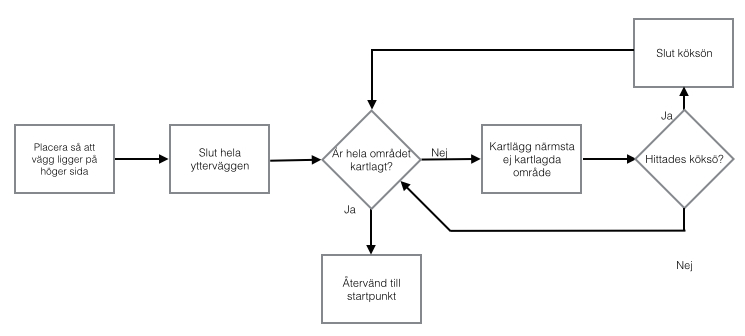
\includegraphics[keepaspectratio=true,scale=0.5]{../../Designspec/Flode_kartritning.jpg}  %skala och filnamn. 
  \end{center}
  \caption{Flödesschema kartläggning} %figurtext.
  \label{fig:fire} %glöm inte att uppdatera era labels
\end{figure}

%------------------------------------------------
%------------Resultat och slutsatser-------------
%------------------------------------------------
\newpage
\section{Resultat och slutsatser}

Till slut kan vi konstatera att SLAM används i många tillämpningar man kanske inte tänker på. Man kan också konstatera att algoritmerna, filtren och mjukvaran som används för att implementera SLAM ibland kan vara väldigt komplexa. I miljöer där sensorerna kan täcka en stor del av banan kan däremot algoritmerna hållas relativt enkla. Detta då variabler med enkelhet kan skattas via avståndssensorernas medelvärde. 

Vi inser att vi gjort ett klokt beslut att fördjupa oss i just SLAM, då vi är beroende av detta i vårt projekt att konstruera en kartritande robot. SLAM var också den delen vi såg, och fortfarande ser, som störst hinder i utvecklingsprocessen. 

Vi har insett att vi tack vare det långa synfältet hos våra optiska sensorer i kombination med det relativt lilla område vi ska kartlägga kommer kunna använda en relativt enkel implementering. En implementering som använder sig av ML-skattning som observatör\footnote{Glad och Ljung (2006)} för systemet. 

% --------------- Källförteckning ---------------------
\newpage 
\section*{Källförteckning} 
\addcontentsline{toc}{section}{Källförteckning}

David Törnqvist. Estimation and Detection with Applications to Navigation. PhD thesis, Linköping University, 2008. Hämtad 15 april 2014.
\url{http://urn.kb.se/resolve?urn=urn:nbn:se:liu:diva-14956}

Datablad Atmega 1284p, Vanheden, databladsserver hos Institutionen för Systemteknik vid Linköpings Universitet. Hämtad 14 april 2014. \url{https://docs.isy.liu.se/twiki/pub/VanHeden/DataSheets/atmega1284p.pdf}

FastSLAM: A Factored Solution to the Simultaneous
Localization and Mapping Problem, Stanford University. Hämtad 28 mars 2014.
\url{http://robots.stanford.edu/papers/montemerlo.fastslam-tr.pdf}

Fox, C.; Evans, M.; Pearson, M.; Prescott, T. (2012)
''Tactile SLAM with a biomimetic whiskered robot''. 2012 IEEE International Conference on Robotics and Automation. Hämtad 28 mars 2014.
\url{http://ieeexplore.ieee.org/stamp/stamp.jsp?tp=&arnumber=6224813}

Glad, Torkel och Ljung, Lennart. 2006. \textit{Reglerteknik - Grundläggande teori}. Upplaga 4:10. Lund. Studentlitteratur AB.

Kandidatprojekt Y: Elektronikprojekt, Tävlingsregler för katläggningsrobot. Hämtad 28 mars 2014.  \url{https://drive.google.com/file/d/0B758zzcy4ZrTeG1wRTY4WG9lTDQ/edit?usp=sharing}

Karlsson, N.; Goncalves, L.; Munich, M.E.; Pirjanian, P.
''The vSLAM Algorithm for Navigation in Natural Environments''. Evolution Robotics, Inc. Hämtad 28 mars 2014:
\url{http://www.vision.caltech.edu/mariomu/research/papers/vSLAM-krs.pdf}

Openslam.org
\url{http://www.openslam.org/}

Risgaard, S; Blas, M.R (2005).
''SLAM for Dummies, A Tutorial Approach to Simultaneous Localization and Mapping''. 
Hämtad 28 mars 2014:
\url{http://ocw.mit.edu/courses/aeronautics-and-astronautics/16-412j-cognitive-robotics-spring-2005/projects/1aslam_blas_repo.pdf}

Smith, R.C.; Cheeseman, P. (1986). ''On the Representation and Estimation of Spatial Uncertainty''. The
International Journal of Robotics Research, 5(4), sida 56–68. Hämtad
28 mars 2014:
\url{http://www.frc.ri.cmu.edu/~hpm/project.archive/reference.file/Smith&Cheeseman.pdf}






\end{document}